\documentclass[12pt]{article}
\usepackage{graphicx}
\usepackage{subcaption}
\usepackage[]{mcode}
\usepackage{mwe}
\usepackage{amsmath}
\usepackage[T1]{fontenc}


\DeclareMathOperator{\erf}{erf}
\renewcommand{\thesubsection}{\thesection.\alph{subsection}}

\begin{document}

\title{CMSC 460 - HW5}
\author{Gudjon Einar Magnusson}

\maketitle

%% 5.5
%x = (9,2,6)
\section{}

%(a) housholder reflection and gibbins rotation
% Hx = (11,0,0)
\subsection{} %a
$x = [9, 2, 6]^T$ 

$H$ is a Householder reflection matrix that gives $Hx = [11, 0, 0]^T$.
\[
H =  
\begin{bmatrix}
    0.8182 & 0.1818 & 0.5455 \\
    0.1818 & 0.8182 & -0.5455 \\
    0.5455 & -0.5455 & -0.6364    
\end{bmatrix}
\]

$G$ is a Givens rotation matrix that gives $Gx = [11, 0, 0]^T$
\[
G =  
\begin{bmatrix}
    0.8182 & 0.1818 & 0.5455 \\
   -0.2169 & 0.9762 & 0 \\
    0.5325 & 0.1183 & -0.8381
\end{bmatrix}
\]

% find u,v s.t Hu = -u, Hv = v
\subsection{} %b
\[
u =  
\begin{bmatrix}
    -1 \\
    0 \\
    0
\end{bmatrix}
\]

\[
v =  
\begin{bmatrix}
    1 \\
    0 \\
    0
\end{bmatrix}
\]

%% 5.7
\section{}

\subsection{} %a

Figure \ref{fig_2a_err} shows that the error drops quickly as the polynomial degree increases.

\begin{figure}
    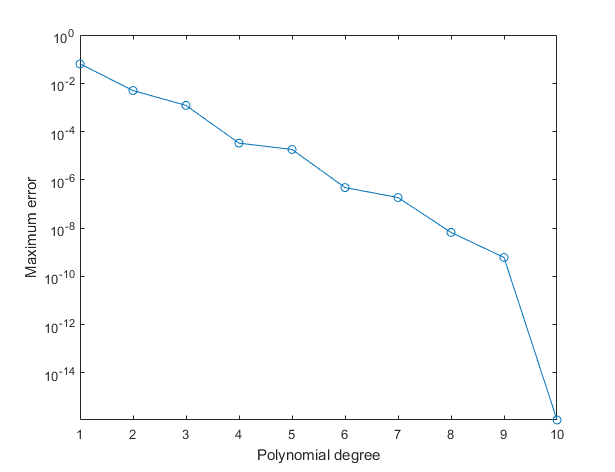
\includegraphics[width=0.6\linewidth]{plot_err}
    \centering
    \caption{}
    \label{fig_2a_err}
\end{figure}

\subsection{} %b

Figure \ref{fig_2b_err} shows that the error grows quickly as the polynomial degree increases. This happens because the polynomial oscillates wildly around the true value.

\begin{figure}
    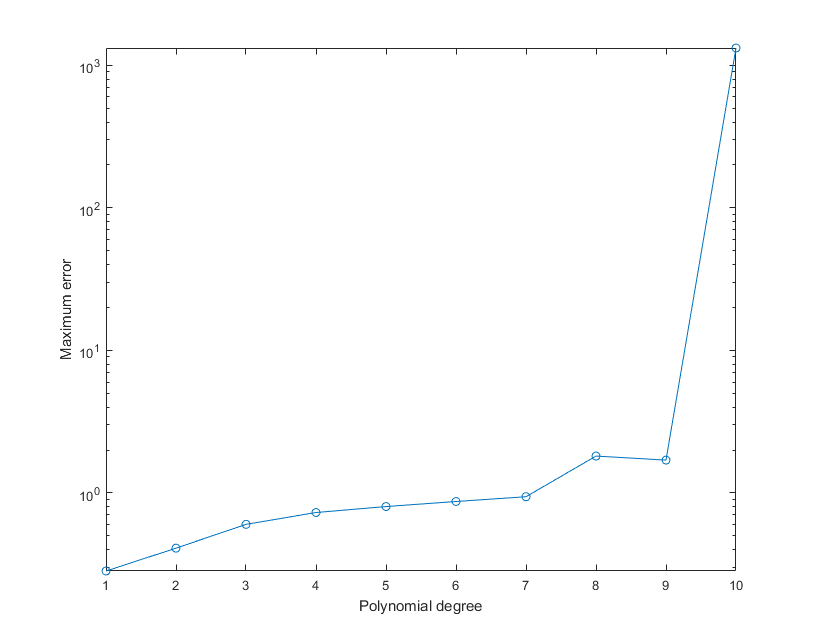
\includegraphics[width=0.6\linewidth]{odd_plot_err}
    \centering
    \caption{}
    \label{fig_2b_err}
\end{figure}

\subsection{} %c

This gives a very good approximation.


%% 5.8
\section{}

\subsection{} %a

Figure \ref{fig_3a_plot} shows the straight line fitted through the data points. Figure \ref{fig_3a_r} shows the residual for each point. The 7th point has a notable larger residual than the rest of the data.

\begin{figure}[t!]
    \begin{subfigure}[t]{0.5\textwidth}
        \centering
        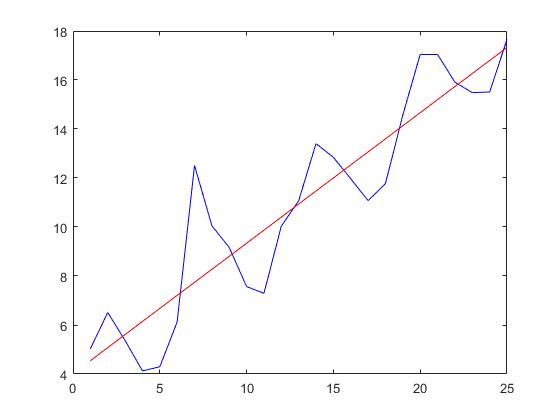
\includegraphics[width=\linewidth]{plot_3a}
        \caption{}
        \label{fig_3a_plot}
    \end{subfigure}
    \begin{subfigure}[t]{0.5\textwidth}
        \centering
        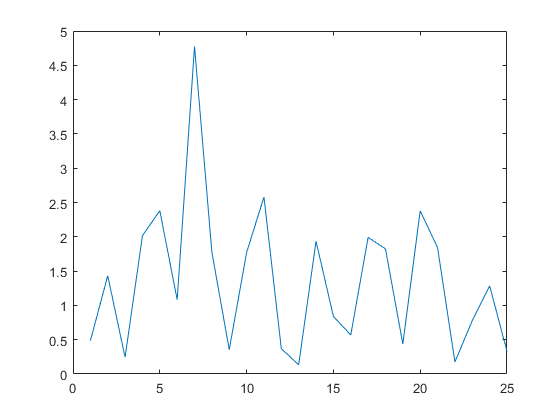
\includegraphics[width=\linewidth]{plot_3a_r}
        \caption{}
        \label{fig_3a_r}
    \end{subfigure}
    \caption{}
    \label{fig_3a}
\end{figure}

\subsection{} %b

Figure \ref{fig_3b_plot} shows the straight line fitted through the data points with the 7th point excluded. Figure \ref{fig_3b_r} shows the residual for each point. The error is now mostly uniform.

\begin{figure}[t!]
    \begin{subfigure}[t]{0.5\textwidth}
        \centering
        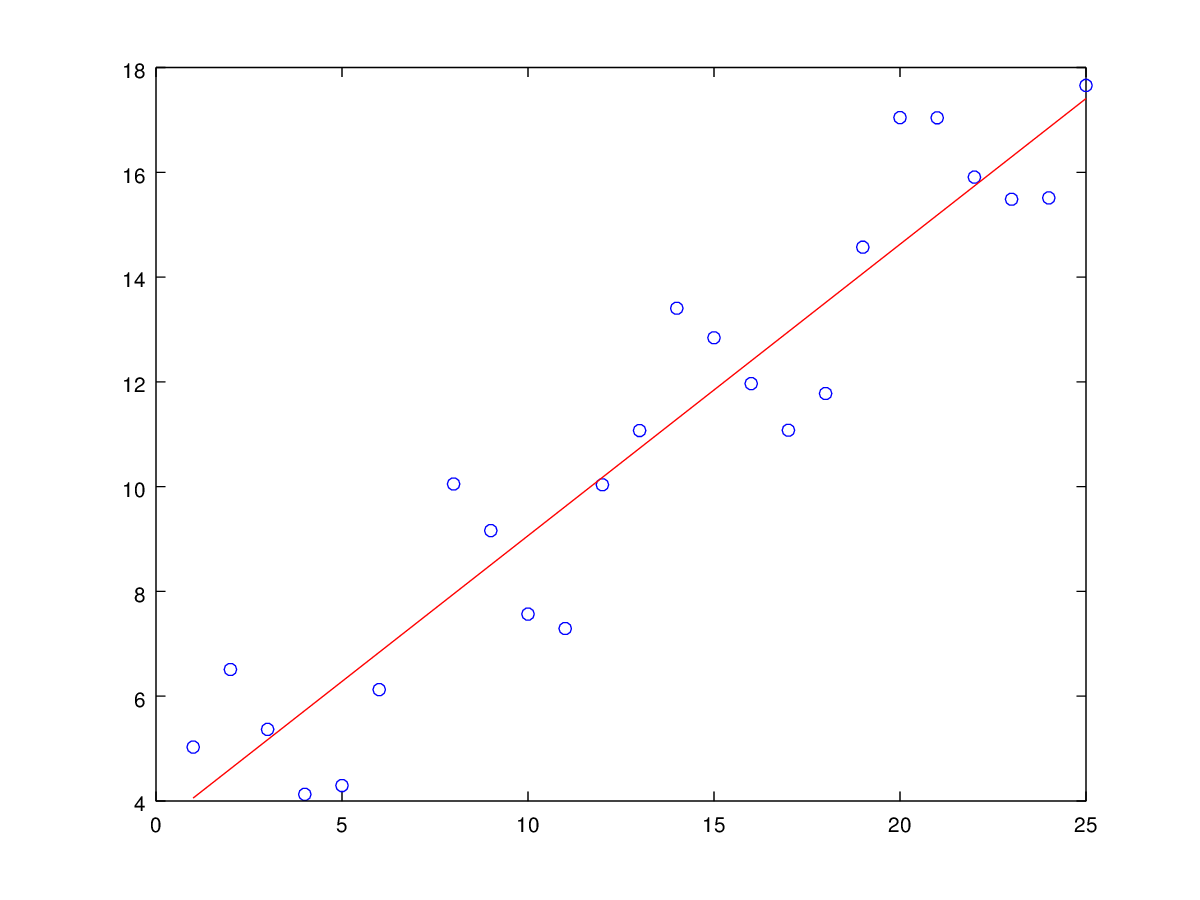
\includegraphics[width=\linewidth]{plot_3b}
        \caption{}
        \label{fig_3b_plot}
    \end{subfigure}
    \begin{subfigure}[t]{0.5\textwidth}
        \centering
        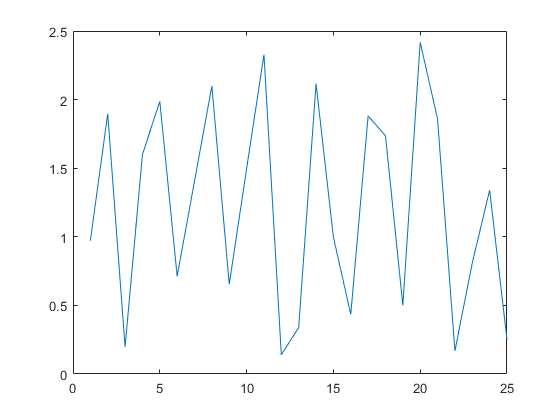
\includegraphics[width=\linewidth]{plot_3b_r}
        \caption{}
        \label{fig_3b_r}
    \end{subfigure}
    \caption{}
    \label{fig_3b}
\end{figure}

\subsection{} %c

Figure \ref{fig_3c_plot} shows the curve line fitted through the data points with the 7th point excluded. Figure \ref{fig_3c_r} shows the residual for each point. The error is now much smaller but less uniform.

\begin{figure}[t!]
    \begin{subfigure}[t]{0.5\textwidth}
        \centering
        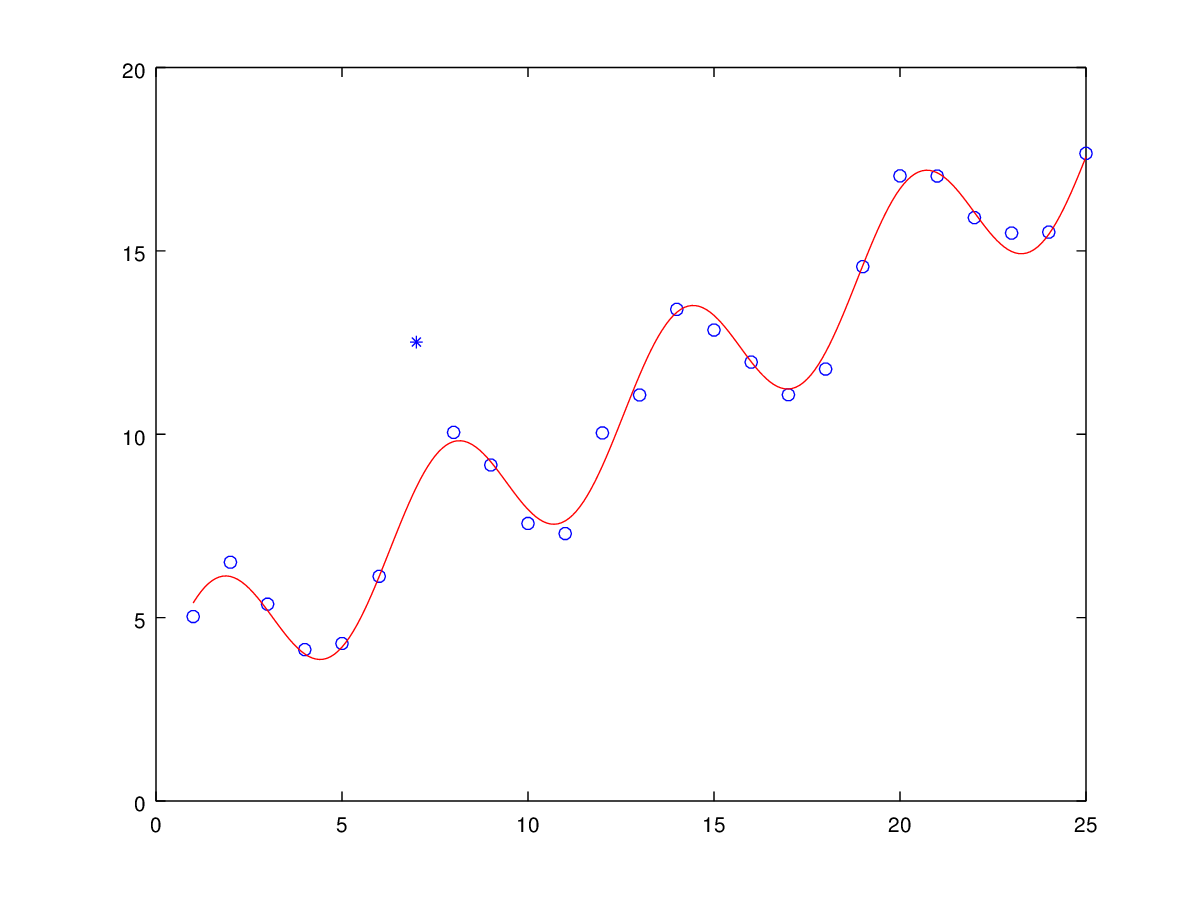
\includegraphics[width=\linewidth]{plot_3c}
        \caption{}
        \label{fig_3c_plot}
    \end{subfigure}
    \begin{subfigure}[t]{0.5\textwidth}
        \centering
        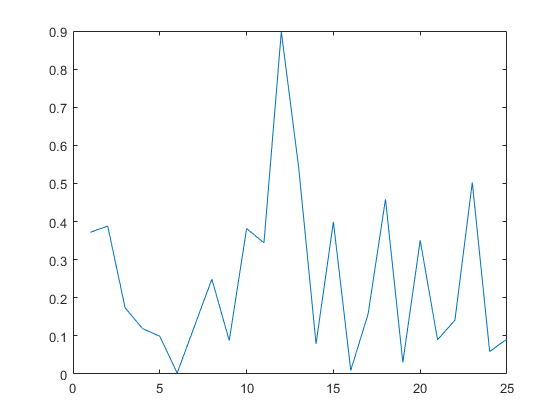
\includegraphics[width=\linewidth]{plot_3c_r}
        \caption{}
        \label{fig_3c_r}
    \end{subfigure}
    \caption{}
    \label{fig_3c}
\end{figure}

%% 5.11
\section{} %3

\subsection{} %a
\begin{minipage}{\linewidth}
\begin{lstlisting}
load longley.dat;
y = longley(:,1);
X = longley(:,2:7);

[m, ~] = size(X);
X = [ones(m,1),X];
b = X\y;


b =    
    1.0e+06 *
      -3.482258634593715
       0.000015061872271
      -0.000000035819179
      -0.000002020229804
      -0.000001033226867
      -0.000000051104106
       0.001829151464612
\end{lstlisting}
\end{minipage}

\subsection{} %b

My values of b match the certified values within a very small error.

\subsection{} %c

Figure \ref{fig_4c} show the value of $y$ according the fitted model. Vertical bars represent the error at each point.

\begin{figure}
    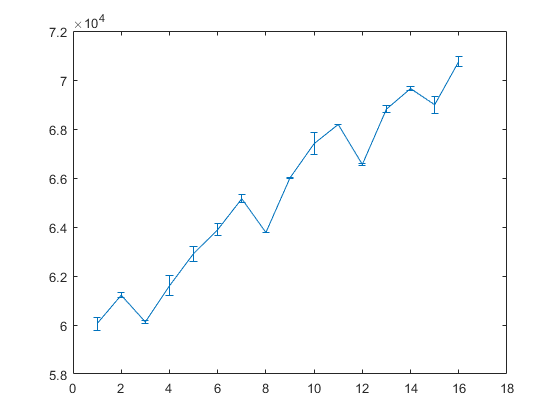
\includegraphics[width=0.6\linewidth]{plot_4c}
    \centering
    \caption{}
    \label{fig_4c}
\end{figure}

\subsection{} %d
There is a strong correlation between unemployment and the size of armed forces.

\begin{minipage}{\linewidth}
\begin{lstlisting}
[R,P,RLO,RUP]=corrcoef(X);

P =
    1.0000    0.0000    0.0103    0.0697    0.0000    0.0000
    0.0000    1.0000    0.0132    0.0830    0.0000    0.0000
    0.0103    0.0132    1.0000    0.5109    0.0033    0.0047
    0.0697    0.0830    0.5109    1.0000    0.1652    0.1078
    0.0000    0.0000    0.0033    0.1652    1.0000    0.0000
    0.0000    0.0000    0.0047    0.1078    0.0000    1.0000
\end{lstlisting}
\end{minipage}

\subsection{} %e

Figure \ref{fig_4e} plots the normalized value of each of the 7 variables.

\begin{figure}
    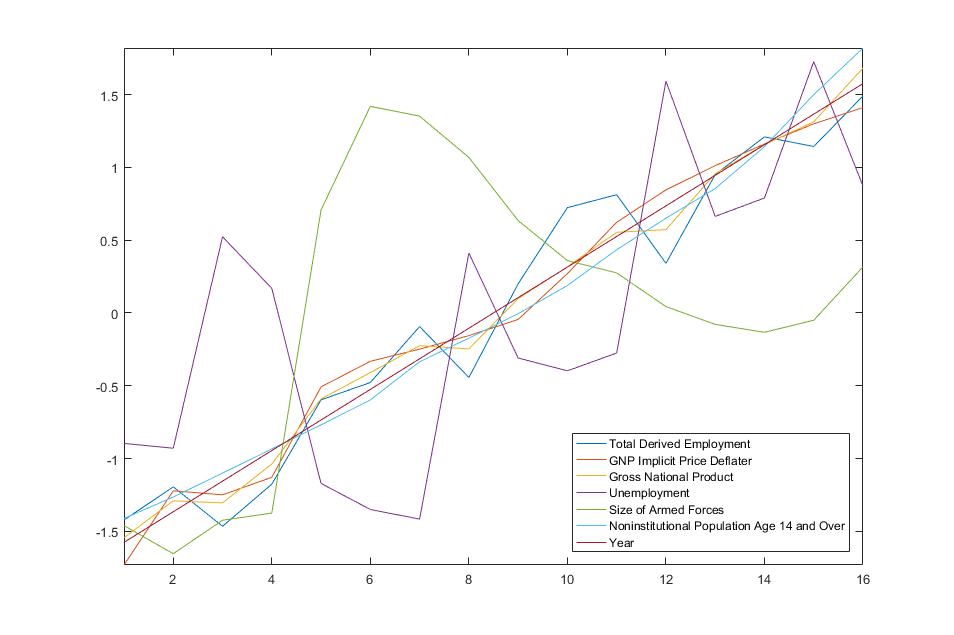
\includegraphics[width=\linewidth]{plot_4e}
    \centering
    \caption{}
    \label{fig_4e}
\end{figure}

\end{document}